\documentclass{scrartcl}


%%% INCLUDE %%%

\usepackage[T1]{fontenc}
\usepackage[utf8]{inputenc}
\usepackage[french]{babel}
\usepackage{layout}
\usepackage{enumitem}
%\usepackage{pifont}
\usepackage{eurosym}
\usepackage{textcomp}
\usepackage{xstring}
%\usepackage{array}
\usepackage{graphicx}

%%% MACRO %%%


% FIXME Prendre en compte les majuscule déjà présente
\makeatletter
\@ifpackageloaded{xstring}{
	\newcommand\smallcaps[1]{\StrLeft{#1}{1}\scriptsize\uppercase{\StrGobbleLeft{#1}{1}}\normalsize }
}{
	\newcommand\smallcaps[1]{\textsc{#1}}
}
\makeatother



%===============================================================================
% Définit un type de puce pour une liste. Si le pakage "pifont" est chargé, il 
% est utilisé, sinon on met un tiret.
\makeatletter
\@ifpackageloaded{pifont}{
	\newcommand\goodItemArrow[0]{\ding{226}}
}{
	\newcommand\goodItemArrow[0]{-}
}
\makeatother



%===============================================================================
% Item de liste avec spécification de la puce et paramètre écrit en gras.
\newcommand\functionality[1]{
	\item[\goodItemArrow] \textbf{#1}\\
}



%===============================================================================
% Commande \Euro indépendante des paquets chargés 
\makeatletter
\@ifpackageloaded{eurosym}{
	\newcommand\Euro[0]{\euro{}}
}{
	\@ifpackageloaded{textcomp}{
		\newcommand\Euro[0]{\texteuro}
	}{
		\newcommand\Euro[0]{Euro}
	}
}
\makeatother



%===============================================================================
% Accès à des variables dans le document. 
%\makeatletter
%\let\titleName\@title
%\let\subtitleName\@subtitle
%\let\authorName\@author
%\makeatother



% Titre de la section courante (que dans beamer)
%\secname 
% Titre de la sous-section courante (que dans beamer)
%\subsecname



% format.tex
% 
% author : Adrien Bisutti
% created : Mon, 26 Oct 2015 16:55:02 +0100
% modified : Mon, 26 Oct 2015 16:55:02 +0100
%

%\usepackage{soul}



%=== Section ===================================================================
% Grand chiffre romain, gras, souligné (FIXME souligné ne marche pas)
\makeatletter
\renewcommand\section{\@startsection {section}{1}{\z@}%
	{-3.5ex \@plus -1ex \@minus -.2ex}%
	{2.3ex \@plus.2ex}%
	{\Large\bfseries\sffamily\underline}}
\makeatother


\renewcommand{\thesection}{\Roman{section}}



%=== Sub-Section ===============================================================
% Chiffre arabe, gras, italique
\makeatletter
\renewcommand\section{\@startsection {section}{1}{\z@}%
	{-3.5ex \@plus -1ex \@minus -.2ex}%
	{2.3ex \@plus.2ex}%
	{\Large\bfseries\sffamily\itshape}}
\makeatother


\renewcommand{\thesubsection}{\arabic{subsection}}



%=== Paragraph =================================================================
% Interligne en dessous de 0.5
% TODO


%=== List ======================================================================
% Interligne en dessous de 1
% TODO


%=== Summary ===================================================================
% mettre des href avec http://www.xm1math.net/doculatex/structure.html
% TODO




%%% DATA %%%

%\title[Cahier des charges]{Surfaces de révolution discrètes}
\title{Surfaces de révolution discrètes}
\subtitle{Cahier des charges}
\author{
	Zied \bsc{Ben Othmane}\\
	Thomas \bsc{Benoist}\\
	Adrien \bsc{Bisutti}\\
	Lydie \bsc{Richaume}
}
%\institute{Université de Poitiers}


\makeatletter
\let\titleName\@title
\let\subtitleName\@subtitle
\let\authorName\@author
\makeatother

% TODO régler le layout



%%% DOCUMENT %%%

\begin{document}


%===============================================================================
%	PAGE DE TITRE
%===============================================================================

\begin{titlepage}
	\vspace*{\stretch{1}}
	
	% --- Titre ---
	\begin{center}
		\fontsize{30}{36}\selectfont\bfseries
		\titleName\\
		\rule{6cm}{0.5pt} % trait horizontal de 6cm de long, 0.5pt d'épaisseur
	\end{center}
	
	% --- Sous-titre ---
	\begin{center}
		\LARGE
		\subtitleName
	\end{center}
	\vspace{1cm}
	
	% --- Auteurs ---
	\begin{center}
		\authorName
	\end{center}
	\vfill
	% --- Logo ---
	\begin{center}
		
\includegraphics[height=3cm]{../Images/logo_univ_poitiers.png}
		\hfill
		
\includegraphics[height=3cm]{../Images/logo-Xlim.png}
	\end{center}
	\vfill
	
	% --- Date ---
	\begin{center}
		\today
	\end{center}
\end{titlepage}
\newpage



%===============================================================================
%	SOMMAIRE
%===============================================================================

\tableofcontents
\newpage



%===============================================================================
%	PRÉSENTATION PROJET
%===============================================================================

%\layout % FIXME
\section{Introduction}


%--- Présentation générale -----------------------------------------------------
	\subsection{Présentation générale du projet}
	Les commanditaires du projet, \'Eric \bsc{Andres} et Gaëlle \bsc{Largeteau-Skapin}, ont développé un nouvel algorithme permettant de générer des surfaces de révolution discrètes. Afin de pouvoir illustrer leurs publications, ils ont fait appel à nous pour développer une application web permettant de générer des surfaces de révolution discrètes à l'aide de leur algorithme.

Nos clients ont également décidé de mettre cette application à disposition de tous, ajoutant un but découverte ou artistique à ce projet initialement scientifique.

%--- Les partis ----------------------------------------------------------------
	\subsection{Les partis}
		Les clients~:
		\begin{itemize}
			\item Éric \bsc{Andres} (Professeur et ancien directeur de département XLIM-SIC)
			\item Gaëlle \bsc{Largeteau-Skapin} (Maitre de Conférence, Géométrie discrète)
		\end{itemize}

		\bigskip % FIXME

		L'équipe de développement~:
		\begin{itemize}
			\item Adrien \bsc{Bisutti}
			\item Lydie \bsc{Richaume}
			\item Thomas \bsc{Benoist}
			\item Zied \bsc{Ben Othmane}
		\end{itemize}


%--- Terminologie --------------------------------------------------------------
	\subsection{Définitions}
		Une surface de révolution est un objet mathématique en trois dimensions généré à l'aide de deux courbes en deux dimensions: la courbe de révolution et la méridienne. La courbe de révolution (le plus souvent un cercle) défini la transformation qui sera appliquée à la méridienne afin de générer la surface de révolution.

%===============================================================================
%	OBJECTIFS CLIENT
%===============================================================================

\section{Objectifs client}

%--- Objectifs application -----------------------------------------------------
	\subsection{Objectifs de l'application et existant}
		L'objectif de ce projet est, d'une part, de proposer un outil simple permettant la génération de surfaces de révolution discrètes et, d'autre part, d'illustrer les publications des clients à ce propos. 

Il existe déjà des solutions efficaces pour générer des surfaces de révolution, cependant le cadre d'un environnement discret ajoute d'importantes contraintes qui ne sont jusqu'à présent pas prises en compte. Actuellement, il est possible de générer des surfaces de révolution discrètes à l'aide d'outils mathématiques (par exemple Mathematica), cependant, cela nécessite un travail important. 

Il n'y a donc actuellement aucun outil qui satisfasse la demande des clients. De plus, la volonté d'illustrer leur travail justifie elle aussi le développement d'une nouvelle application.


	\subsection{Expression des besoins}
		L'application devra proposer les possibilités suivantes~:
		\begin{itemize}[label={*}]
			\item Définir la méridienne et la courbe de révolution
			\begin{itemize}[label={-}]
				\item Choisir dans des listes de courbes prédéfinies
				\item Entrer une équation
				\item Dessiner à la main (seulement pour la méridienne)
			\end{itemize}
			\item Générer la surface de révolution correspondante
			\item Exporter les surfaces générées
			\begin{itemize}[label={-}]
				\item Pour un modeleur
				\item Pour une imprimante 3D
			\end{itemize}
		\end{itemize}

%--- Exigences clients ---------------------------------------------------------
	\subsection{Exigences client}
		Selon les termes des clients, l'application devra être accessible et utilisable par tous. Cela donnera lieu à une application web ayant une interface simple d'utilisation.

%	\subsection{Analyse des besoins}



%===============================================================================
%	Objectifs techniques
%===============================================================================
			
\section{Spécifications techniques}		

%--- Exigences techniques ------------------------------------------------------
	\subsection{Proposition technologiques}
		Le projet est réalisé avec les technologies WebGL, basées sur le JavaScript pour la partie modélisation.
		La partie interface utilisera HTML 5, CSS 3 et jQuery. 
		Les développeurs se réservent le droit d'utiliser d'autres bibliothèques, sous licence libre, afin de développer toutes les fonctionnalités.


%--- Fonctionnalités -----------------------------------------------------------
	\subsection{Fonctionnalités}
		Les différentes fonctionnalités que proposera l'application finale peuvent être regroupées en fonctionnalités plus générales~:			
		
		\medskip % FIXME
		
		\begin{itemize}
			\item Génération des surfaces
			\item Manipulation de l'espace 3D
			\item Gestion des courbes 2D
			\item Export des données
			\item Sauvegarde des données
		\end{itemize}
	
		\bigskip % FIXME
		
		Une liste détaillée des fonctionnalités est disponible en annexe dans le fichier \emph{Listes de fonctionnalités.pdf}.

%--- Interface -----------------------------------------------------------------
	\subsection{Interface}
		L'interface de l'application proposera trois espaces de visualisation~:
			
			\begin{itemize}
				\item Un espace pour visualiser la méridienne et la dessiner à main levée
				\item Un espace pour visualiser la courbe de révolution
				\item Un espace pour visualiser la surface générée
			\end{itemize}
			
		Chaque espace sera accompagné d'un menu contenant les options correspondantes.\\
		Pour les courbes~:			
		\begin{itemize}
			\item Choix parmi une liste de la façon de définir la courbe (courbe prédéfinie, formule, dessin)
			\item Pour une courbe prédéfinie~:
			\begin{itemize}[label={*}]
				\item Choix de la courbe parmi une liste
				\item Réglage des paramètres de la courbe (par exemple la pente et l'ordonnée à l'origine pour une courbe affine)
			\end{itemize}
			\item Pour une formule~:
			\begin{itemize}[label={*}]
				\item Un ou plusieurs champs pour entrer les formules
			\end{itemize}
			\item Des options de sauvegarde
		\end{itemize}
		
		Pour l'espace 3D~:
		
		\begin{itemize}
			\item Des sliders pour gérer les vues en coupe
			\item Un outil permettant de gérer la taille de la grille
			\item Un bouton de génération
			\item Des options d'export
		\end{itemize}
		
		Des options avancées (par exemple la taille d'affichage des voxels) seront aussi disponibles mais restent à définir.
		
		Un exemple de l'interface envisagée est présentée en annexe.


%--- Export --------------------------------------------------------------------
	\subsection{Exports}
		L'application proposera au moins deux formats d'export~: un format pour les modeleurs 3D (exemple~: x3d) et un format pour les imprimantes 3D (exemple~: stl).
		
		Il sera également possible d'exporter des images des courbes et de la surface générée.



%--- Contraintes ---------------------------------------------------------------			
	\subsection{Contraintes}
		Le projet aboutira à une application utilisable sur le web, cependant l'hébergément et la mise en ligne de l'application sera laissée à la charge des clients.
		
		Cette application doit être facile à prendre en main mais doit également proposer des options avancées. Ces dernières devront permettre à un utilisateur prêt à passer plus de temps sur la manipulation de l'application d'utiliser ses connaissances en mathématiques pour définir plus précisément sa surface de révolution. Ces options seront définies plus précisément avec le client au cours du projet.



%===============================================================================
%	RÉALISATION
%===============================================================================

\section{Organisation du projet}


	\subsection{Méthodes développement}
		Ce projet sera réalisé suivant une méthode de développement en spirale.
		\`A chaque fin de cycle, une réunion aura lieu pour discuter avec les clients du livrable produit.
	
%--- Contraintes des partis ----------------------------------------------------
	\subsection{Contraintes des partis}
		Les développeurs s'engagent à~:
			
		\medskip
		
		\begin{itemize}
			\item fournir une application minimale fonctionnelle
			\item fournir une application utilisable par tous
			\item fournir une application utilisable hors-ligne
			\item fournir une application utilisable sur firefox 32 ou superieur
			\item développer une application maintenable et évolutive
			\item fournir une documentation d'aide à l'utilisation de l'application
		\end{itemize}
		
		\bigskip % FIXME sale !
		
		Les clients s'engagent à~:
			
		\medskip
		
		\begin{itemize}
			\item fournir l'algorithme de génération des surfaces de révolution
			\item fournir les outils (git, trac) et le matériel nécessaires au fonctionnement du projet
			\item participer, si possible, aux réunions de fin de cycle
			\item assister aux prestation suivantes~:
				\begin{itemize} 
					\item[\textasteriskcentered] réunion de lancement
					\item[\textasteriskcentered] réunion de revue de projet
					\item[\textasteriskcentered] livraison
					\item[\textasteriskcentered] soutenance finale
				\end{itemize}
			\item répondre aux questions concernant les algorithmes ou les choix d'interface
			\item tester les livrables fournis à chaque fin de cycle et effectuer un retour
		\end{itemize}  


%--- Ressources ----------------------------------------------------------------
	\subsection{Ressources}
		L'équipe de développement devra disposer de quatre machines. Ces quatre machines devront être capable d'exécuter une application WebGL de manière fluide.
		Deux de ces machines seront équipées de Windows 7 ou Windows 10 et deux autres seront équipées d'Ubuntu 12.04 ou ultérieur.

		Sur chacune des machines, les logiciels suivants devront être installés~:
		\medskip
		
		\begin{itemize}
			\item Git
			\item Firefox 32 ou ultérieur
			\item WebGL
			\item Firebug
			\item JsDoc
			\item Notepad++ (seulement pour Windows)
			\item Gedit avec le paquet \emph{gedit-plugins} (seulement pour Ubuntu)
		\end{itemize}



%--- Tests ---------------------------------------------------------------------
	\subsection{Tests et plan d'assurance qualité logiciel}
		Chaque fin de cycle, l'application sera testée par les développeurs. Le choix du ou des programmes de test est laissé à l'équipe de développement. Une fois le cycle terminé et le jalon atteint, les clients devront effectuer la validation des fonctionnalités fournies pour chaque livrables. Ces tests seront effectués selon la norme ISO-9126.

			
\newpage
%--- Échéances et livrables -----------------------------------------------------		
	\subsection{Échéances et livrables}
		\`A chaque fin de cycle, une version fonctionnelle de l'application sera fournie avec des fonctionnalités additionelles. Ces fonctionnalités seront accompagnées de documentation.
		
		Le livrable final contiendra l'application fonctionnelle avec toutes les fonctionnalités minimales décrites dans les spécifications techniques, les documents techniques et le code source.
		
		Les livrables seront les suivants~:\\
		\begin{tabular}{|c|c|p{4cm}|p{7.5cm}|} % FIXME sale !!! FIXME la tableau doit tenir sur la feuille !
			\hline
			\textbf{\No} & \textbf{Date} & \textbf{Type}&\textbf{Description} \\
			\hline
			1 & 23/12 & 
			\begin{itemize}
				\item logiciel
				\item aide utilisateur
				\item documentation technique
			\end{itemize}& 
			\begin{itemize}
				\item génération de surfaces à partir de courbes prédéfinies
				\item une seule méridienne et une seule courbe de révolution non modifiables
				\item interface minimale
			\end{itemize} \\
			\hline
			2 & 21/01& 
			\begin{itemize}
				\item logiciel
				\item aide utilisateur
			\end{itemize}& 
			\begin{itemize}
				\item choix des méridiennes et courbes de révolution à l'aide de listes
				\item possibilité de naviguer et d'afficher des coupes dans l'espace 3D
			\end{itemize} \\
			\hline
			3 & 29/01 &
			\begin{itemize}
				\item logiciel
				\item aide utilisateur
			\end{itemize}& 
			\begin{itemize}
				\item paramètres simple pour les courbes prédéfinies
				\item tracé à main levée pour la méridienne
			\end{itemize} \\
			\hline
			4 & 19/02 &
			\begin{itemize}
				\item logiciel
				\item aide utilisateur
			\end{itemize}& 
			\begin{itemize}
				\item paramètres avancés
				\item possibilité d'entrer une formule pour définir une courbe
				\item export et sauvegarde
			\end{itemize} \\
			\hline
			5 & 2/03 &\begin{itemize}
				\item logiciel
				\item aide utilisateur
				\item documentation technique
			\end{itemize}&
			\begin{itemize}\item Application finale\end{itemize}\\
			\hline
		\end{tabular}


%--- Communications ------------------------------------------------------------
	\subsection{Communications}
		La communication se fera selon différents moyens~:
			\begin{itemize}
				\item mails
				\item réunions
			\end{itemize}
			
		Il y aura, si possible, une réunion avec les clients à chaque début de cycle. Les partis se réservent le droit de demander des entretiens supplémentaires.



%===============================================================================
%	COÛTS
%===============================================================================

\section{Coûts}
	Le coût total du projet est fixé 40 000\Euro{}. Cette somme sera réglée en plusieurs fois sur toute la durée de la phase de réalisation. À l'issue du premier jalon offrant le premier livrable, 30\% de la somme sera versé (soit 12 000\Euro{}). Chaque jalon suivant sera accompagné d'un versement de 10\% (soit 4 000\Euro{}) ou du versement du reste de la somme pour le dernier jalon.



%===============================================================================
%	ANNEXE
%===============================================================================
\newpage
\section*{Annexe}

	\begin{figure}[!h]
		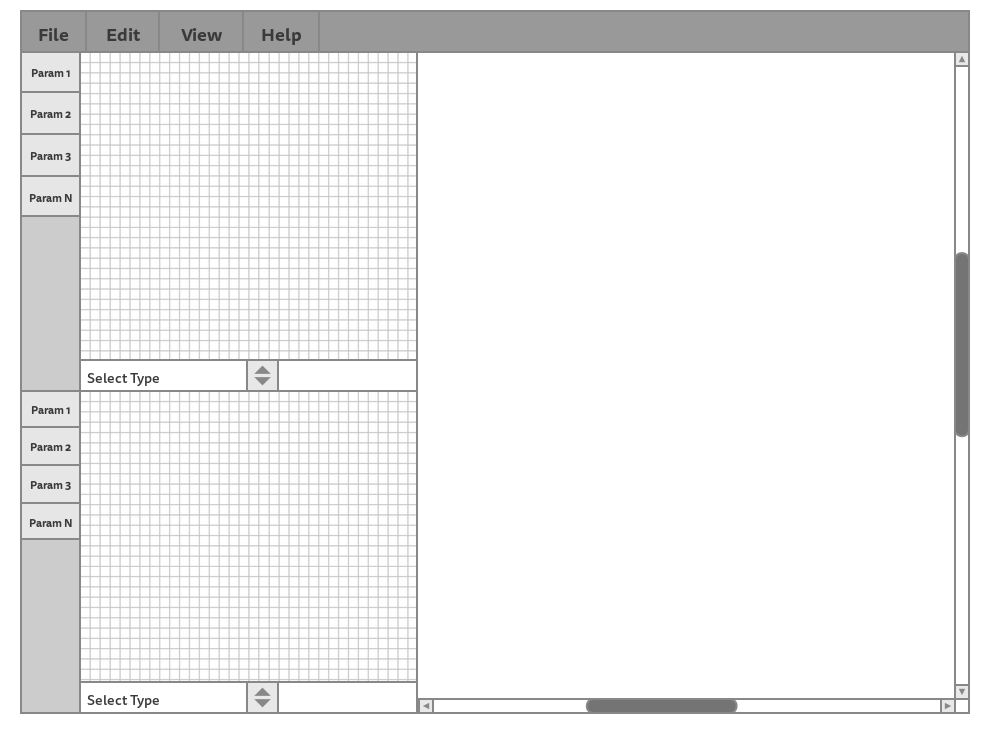
\includegraphics[width=\textwidth]{../Images/example_ihm.png}
		\caption{Exemple d'interface.}
	\end{figure}

\end{document}

